% -------------- TABLA PARA REQUERIMIENTOS FUNCIONALES ---------------- %
% Nomenclatura para la prioridad:
%	MA - Muy Alta
%	A - Alta
%	M - Media
%	B - Baja
%	MB - Muy Baja

\begin{table}[htbp!]
    \begin{requerimientos}

        \FRitem{RM1}{Registrar Mapa Curricular}{El Usuario Miembro de la Comisión puede registrar los datos del Mapa Curricular acorde al \hyperref[MD-SP4]{Modelo de Datos}.}{A}{Origen}
        \label{RM1}

        \FRitem{RM2}{Registrar Unidad de Aprendizaje}{El sistema debe permitir ingresar los datos de las Unidades de Aprendizaje que componen al Mapa Curricular acorde al \hyperref[MD-SP4]{Modelo de Datos}.}{A}{Origen}
        \label{RM2}

        \FRitem{RM3}{Finalizar Mapa Curricular}{El sistema debe permitir finalizar el registro del Mapa  Curricular.}{A}{Origen}
        \label{RM3}

        \FRitem{RM4}{Guardar Mapa Curricular}{El sistema debe permitir guardar el estado actual del Mapa Curricular .}{M}{Origen}
        \label{RM4}

        \FRitem{RM5}{Consultar Mapa Curricular }{El sistema debe permitir visualizar la totalidad de los contenidos del Mapa Curricular registrados.}{M}{Origen}
        \label{RM5}

        \FRitem{RM6}{Editar Mapa Curricular }{El sistema debe permitir modificar la información general del Mapa Curricular.}{M}{Origen}
        \label{RM6}

        \FRitem{RM7}{Eliminar Unidad de Aprendizaje }{El sistema debe permitir eliminar las Unidades de Aprendizaje registradas.}{M}{Origen}
        \label{RM7}

        \FRitem{RM8}{Gestionar dependencias de Unidad de Aprendizaje}{ El Sistema debe permitir la gestión de las dependencias entre las Unidades de Aprendizaje.}{M}{Origen}
        \label{RM8}

        \FRitem{RM9}{Validar congruencia en el Mapa Curricular}{ El Sistema validará la congruencia de los datos registrados.}{M}{Origen}
        \label{RM9}

        \FRitem{RM10}{Aprobar Mapa Curricular}{el Sistema debe permitirle al Usuario Jefe  de Innovación Educativa aprobar el Mapa Curricular.}{M}{Origen}
        \label{RM10}

        \FRitem{RM11}{Enviar Comentarios}{ El Sistema debe permitirle al Usuario Jefe de Innovación Educativa enviar comentarios de corrección sobre el Mapa Curricular.}{M}{Origen}
        \label{RM11}

        \FRitem{RM12}{Visualizar Comentarios}{ El Sistema debe permitirle al Usuario Miembro de la Comisión visualizar comentarios hechos al Mapa Curricular, tanto por el Departamento de Innovación Educativa como por la DES.}{M}{Origen}
        \label{RM12}

        \FRitem{RM13}{Modificar Unidad de Aprendizaje }{El sistema debe permitir hacer modificaciones a cualquiera de las Unidades de Aprendizaje registradas.}{B}{Origen}
        \label{RM13}


    \end{requerimientos}
    \caption{Requerimientos funcionales del sistema para el subproceso de elaboración del Mapa Curricular}
    \label{tbl:RFUA}
\end{table}

\begin{figure}[htbp]
    \begin{center}
        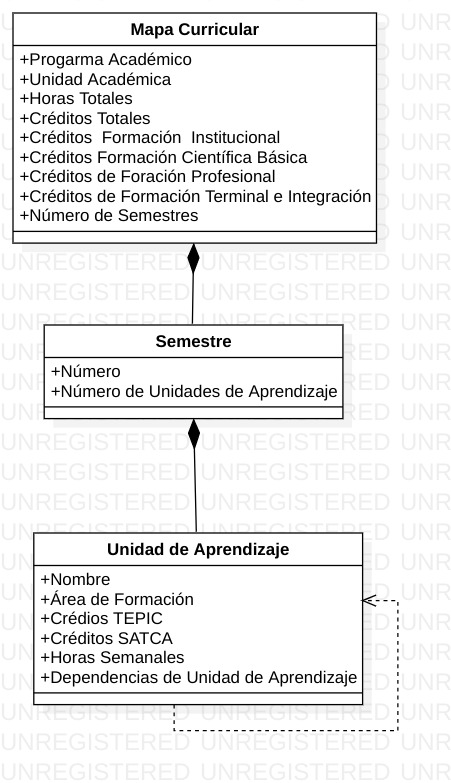
\includegraphics[width=.50\textwidth]{C2-DR/SP4/Image/ModeloDeDatosMC}
        \label{MD-SP4}
        \caption{Modelo de Datos Subproceso para la  Carga del Mapa Curricular}
    \end{center}
\end{figure}

\begin{figure}[htbp]
	\begin{center}
		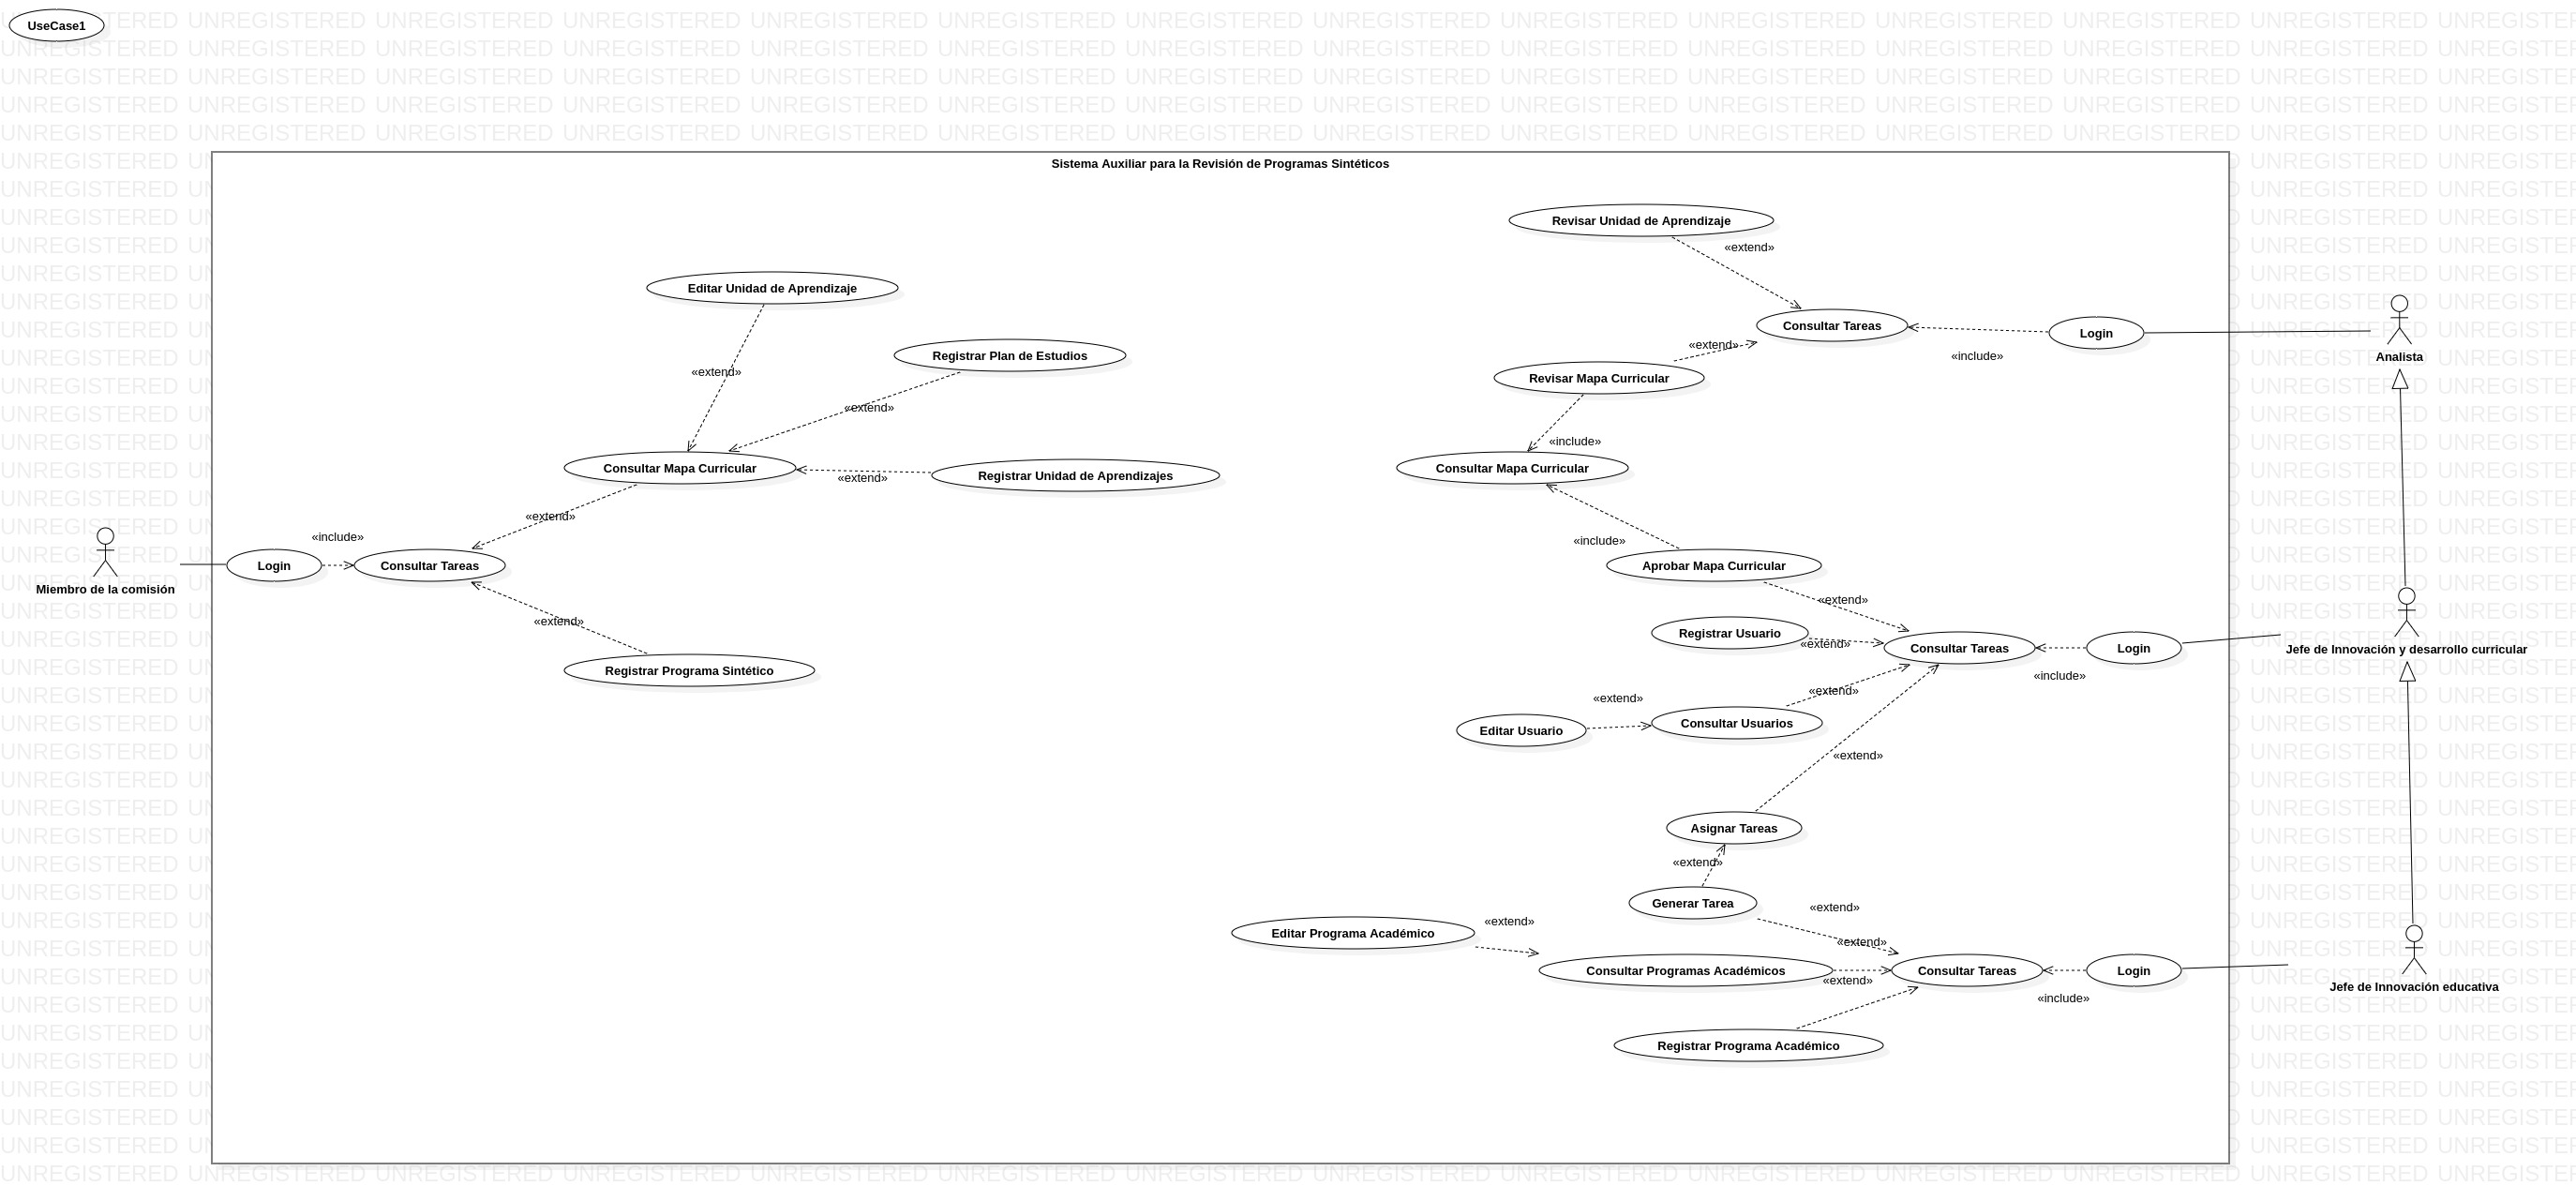
\includegraphics[width=.95\textwidth]{C2-DR/SP4/Image/CasosDeUso}
		\caption{Casos de Uso Subproceso para la  Carga del Mapa Curricular}
		\label{CU-SP4}
	\end{center}
\end{figure}

\begin{center}
	\begin{tabular}{|c|c|c|c|}
		\hline
		ID & Caso de uso & Requerimientos & Encargado \\ \hline
        1 & Registrar Mapa Curricular & \hyperref[RM1]{RM1} & Josué \\ \hline
        2 & Guardar Mapa Curricular & \hyperref[RM4]{RM4} & Andrés \\ \hline
        3 & Consultar Mapa Curricular & \hyperref[RM5]{RM5} & Arturo \\ \hline
		4 & Editar Información General & \hyperref[RM6]{RM6} & Josué \\ \hline
        5 & Finalizar Mapa Curricular & \hyperref[RM3]{RM3} & Josué \\ \hline
        6 & Aprobar Mapa Curricular & \hyperref[RM11]{RM11} & Andrés \\ \hline
        7 & Registrar Unidades de Aprendizaje & \hyperref[RM2]{RM2} & Arturo \\ \hline
        8 & Editar Unidades de Aprendizaje & \hyperref[RM8]{RM8} & Andrés \\ \hline
        9 & Eliminar Unidades de Aprendizaje & \hyperref[RM7]{RM7} & Arturo \\ \hline
        10 & Registrar Dependencias & \hyperref[RM9]{RM9} & Andrés \\ \hline
        11 & Editar Dependencias & \hyperref[RM9]{RM9} & Josué \\ \hline
        12 & Eliminar Dependencias & \hyperref[RM9]{RM9} & Arturo \\ \hline
        13 & Visualizar Comentarios & \hyperref[RM13]{RM13} & Josué \\ \hline
        14 & Enviar Comentarios & \hyperref[RM12]{RM12} & Andrés \\ \hline
    \end{tabular}
\end{center}
